\documentclass[12pt,a4paper,fleqn]{article}
\title{Progress Report}
\author{Syed Ahmad Raza}
\date{2018.06.13}
\usepackage{mathtools}      % for math
\usepackage{graphicx}       % for graphics
%\usepackage{xcolor}         % for using colors in document
%\usepackage{afterpage}
\usepackage{float}          % force a figure placement with [H] command
%\usepackage{enumitem}       % control layout of itemize and enumerate
\usepackage{newtxtext}      % better text font
\usepackage{newtxmath}      % better math font
\usepackage{nicefrac}       % use nicer smaller fractions
%\usepackage{layouts}       % find \printinunitsof{in}\prntlen{\textwidth}
\graphicspath{{../figures/}}% only works when -shell-escape option is used

\begin{document}
\maketitle
%\tableofcontents
%\pagebreak

\section{Validation of 3D Navier-Stokes Solver using QUICK scheme}

A three-dimensional finite volume Navier-Stokes solver was coded in C++. Results were obtained for three-dimensional lid-driven cubic cavity flowusing QUICK scheme with \(\text{Re}=100\) for a 41\(\times\)41\(\times\)41 grid size. The pressure contours and velocity vectors are shown below.

\begin{figure}[H]
    \centering
    \includegraphics[width=\linewidth]{3DPressure.png}
    \caption{Pressure contours for three-dimensional cavity flow}
\end{figure}

\begin{figure}[H]
    \centering
    \includegraphics[width=\linewidth]{3DVelVectors.png}
    \caption{Velocity vectors for three-dimensional cavity flow}
\end{figure}

\subsection{Comparison with published literature}
The simulation results at \(\text{Re}=100\) have been compared with the published results of Ku et al. \cite{Ku:1987:PMS:33136.33145} for three-dimensional cubic cavity flow and Ghia et al. \cite{GHIA1982387} for two-dimensional square cavity flow. The figures below represent the comparison of \(x\)-direction velocity \(u\) on the vertical centerline and \(y\)-direction velocity \(v\) on the horizontal centerline of the cubic cavity.

\begin{figure}[H]
    \centering
    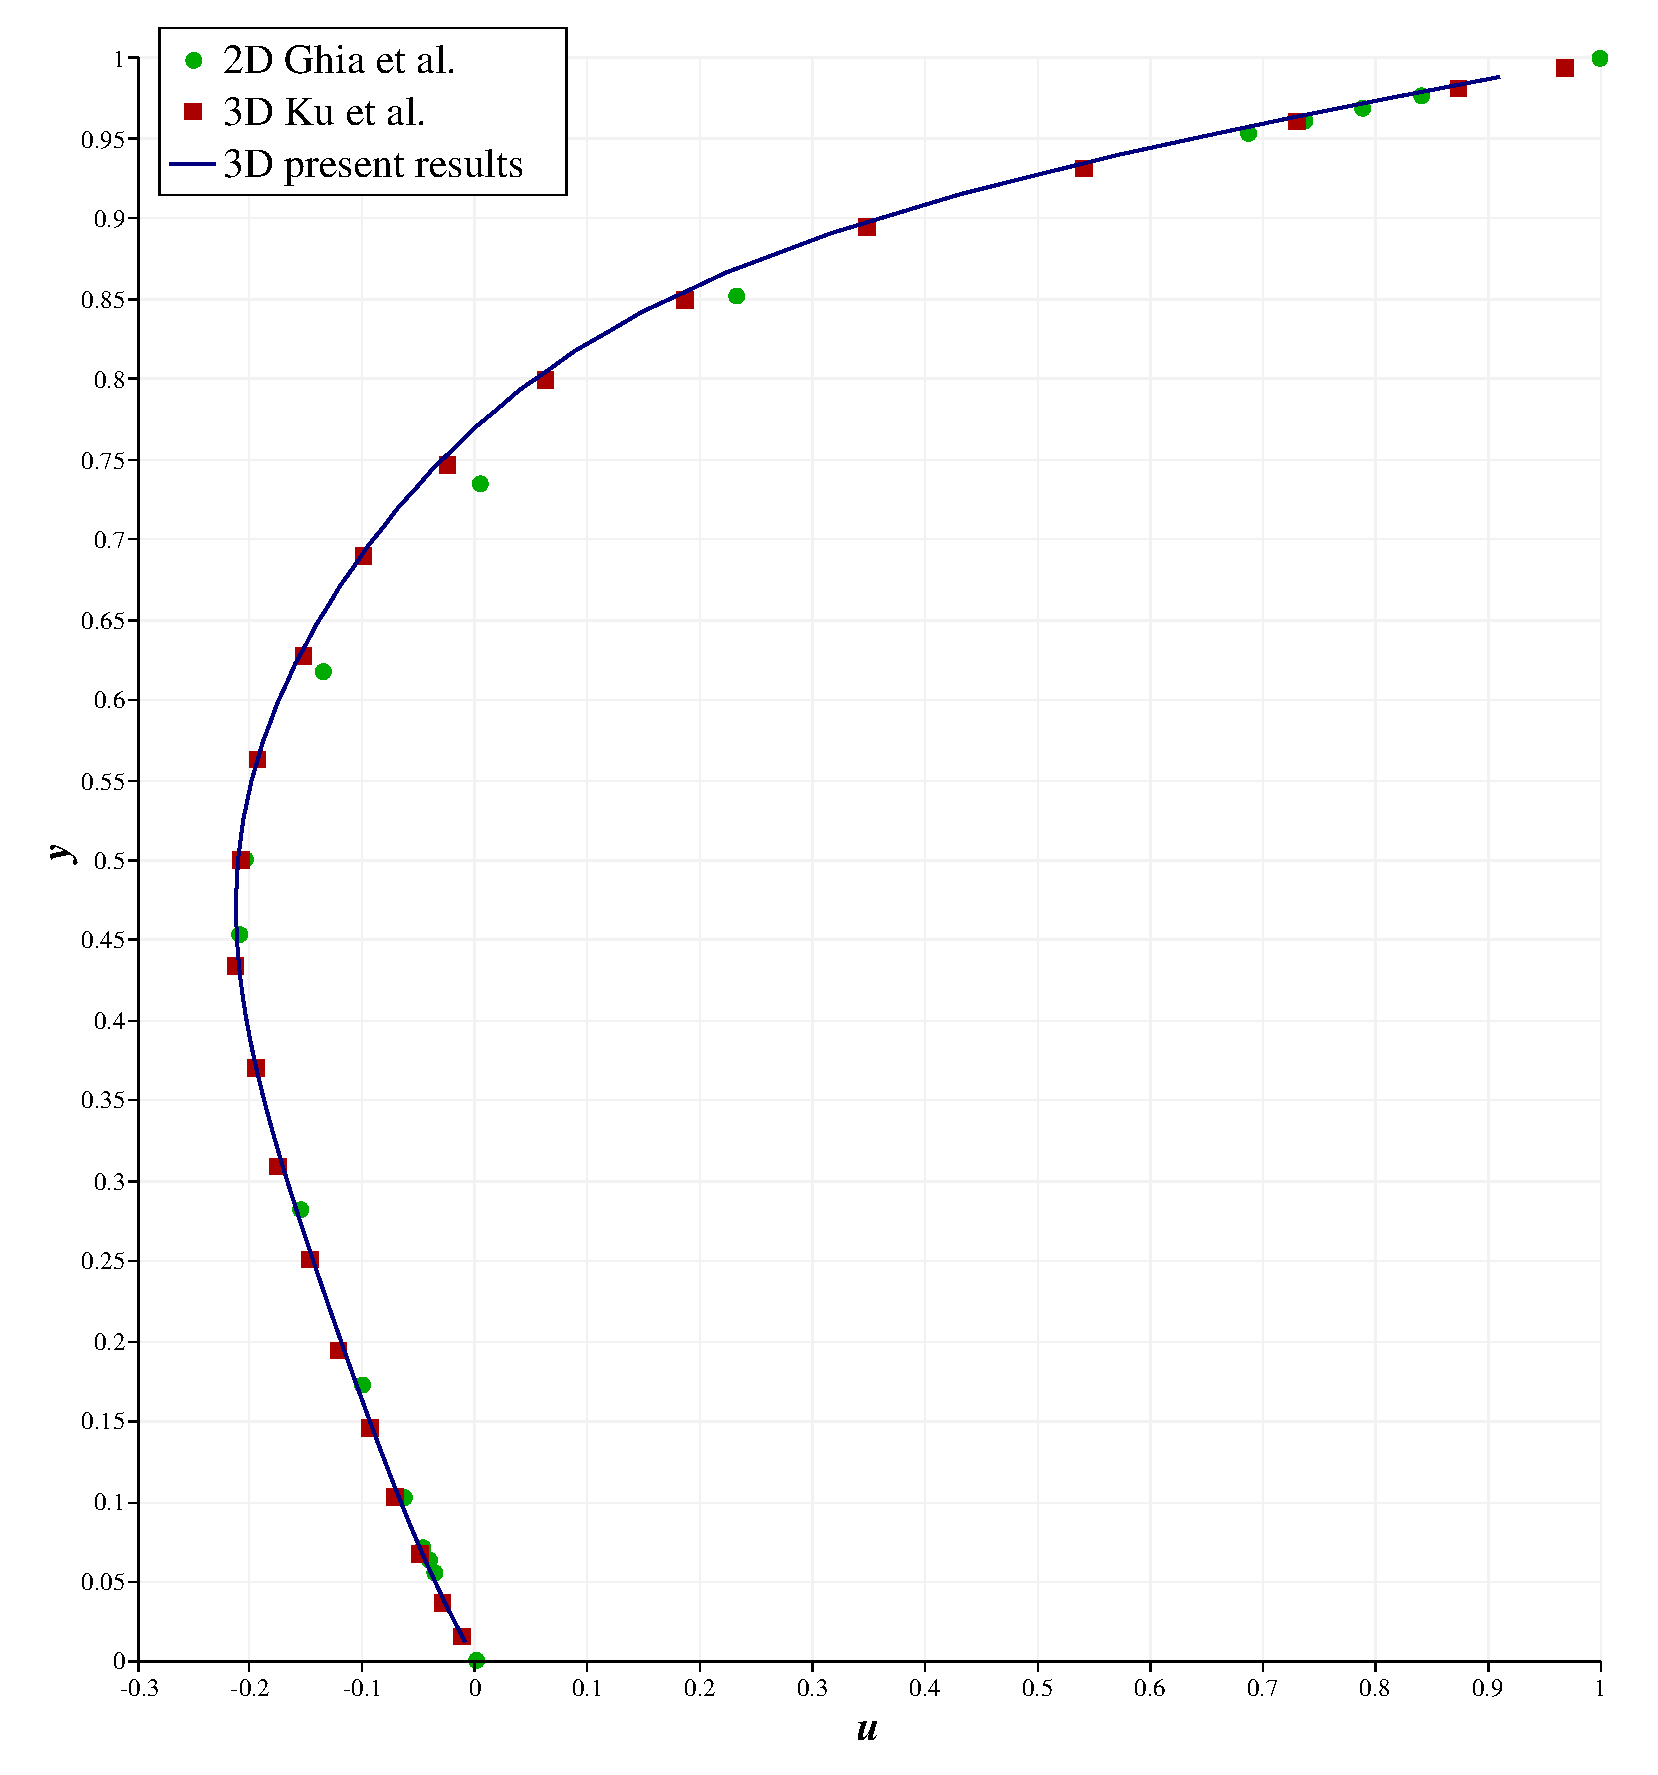
\includegraphics[width=\linewidth]{U-3D_vs_Ku-3D.eps}
    \caption{\(u\)-velocity profile on the vertical centerline in cubic cavity (at the center of \(z\)-axis).}
\end{figure}

\begin{figure}[H]
    \centering
    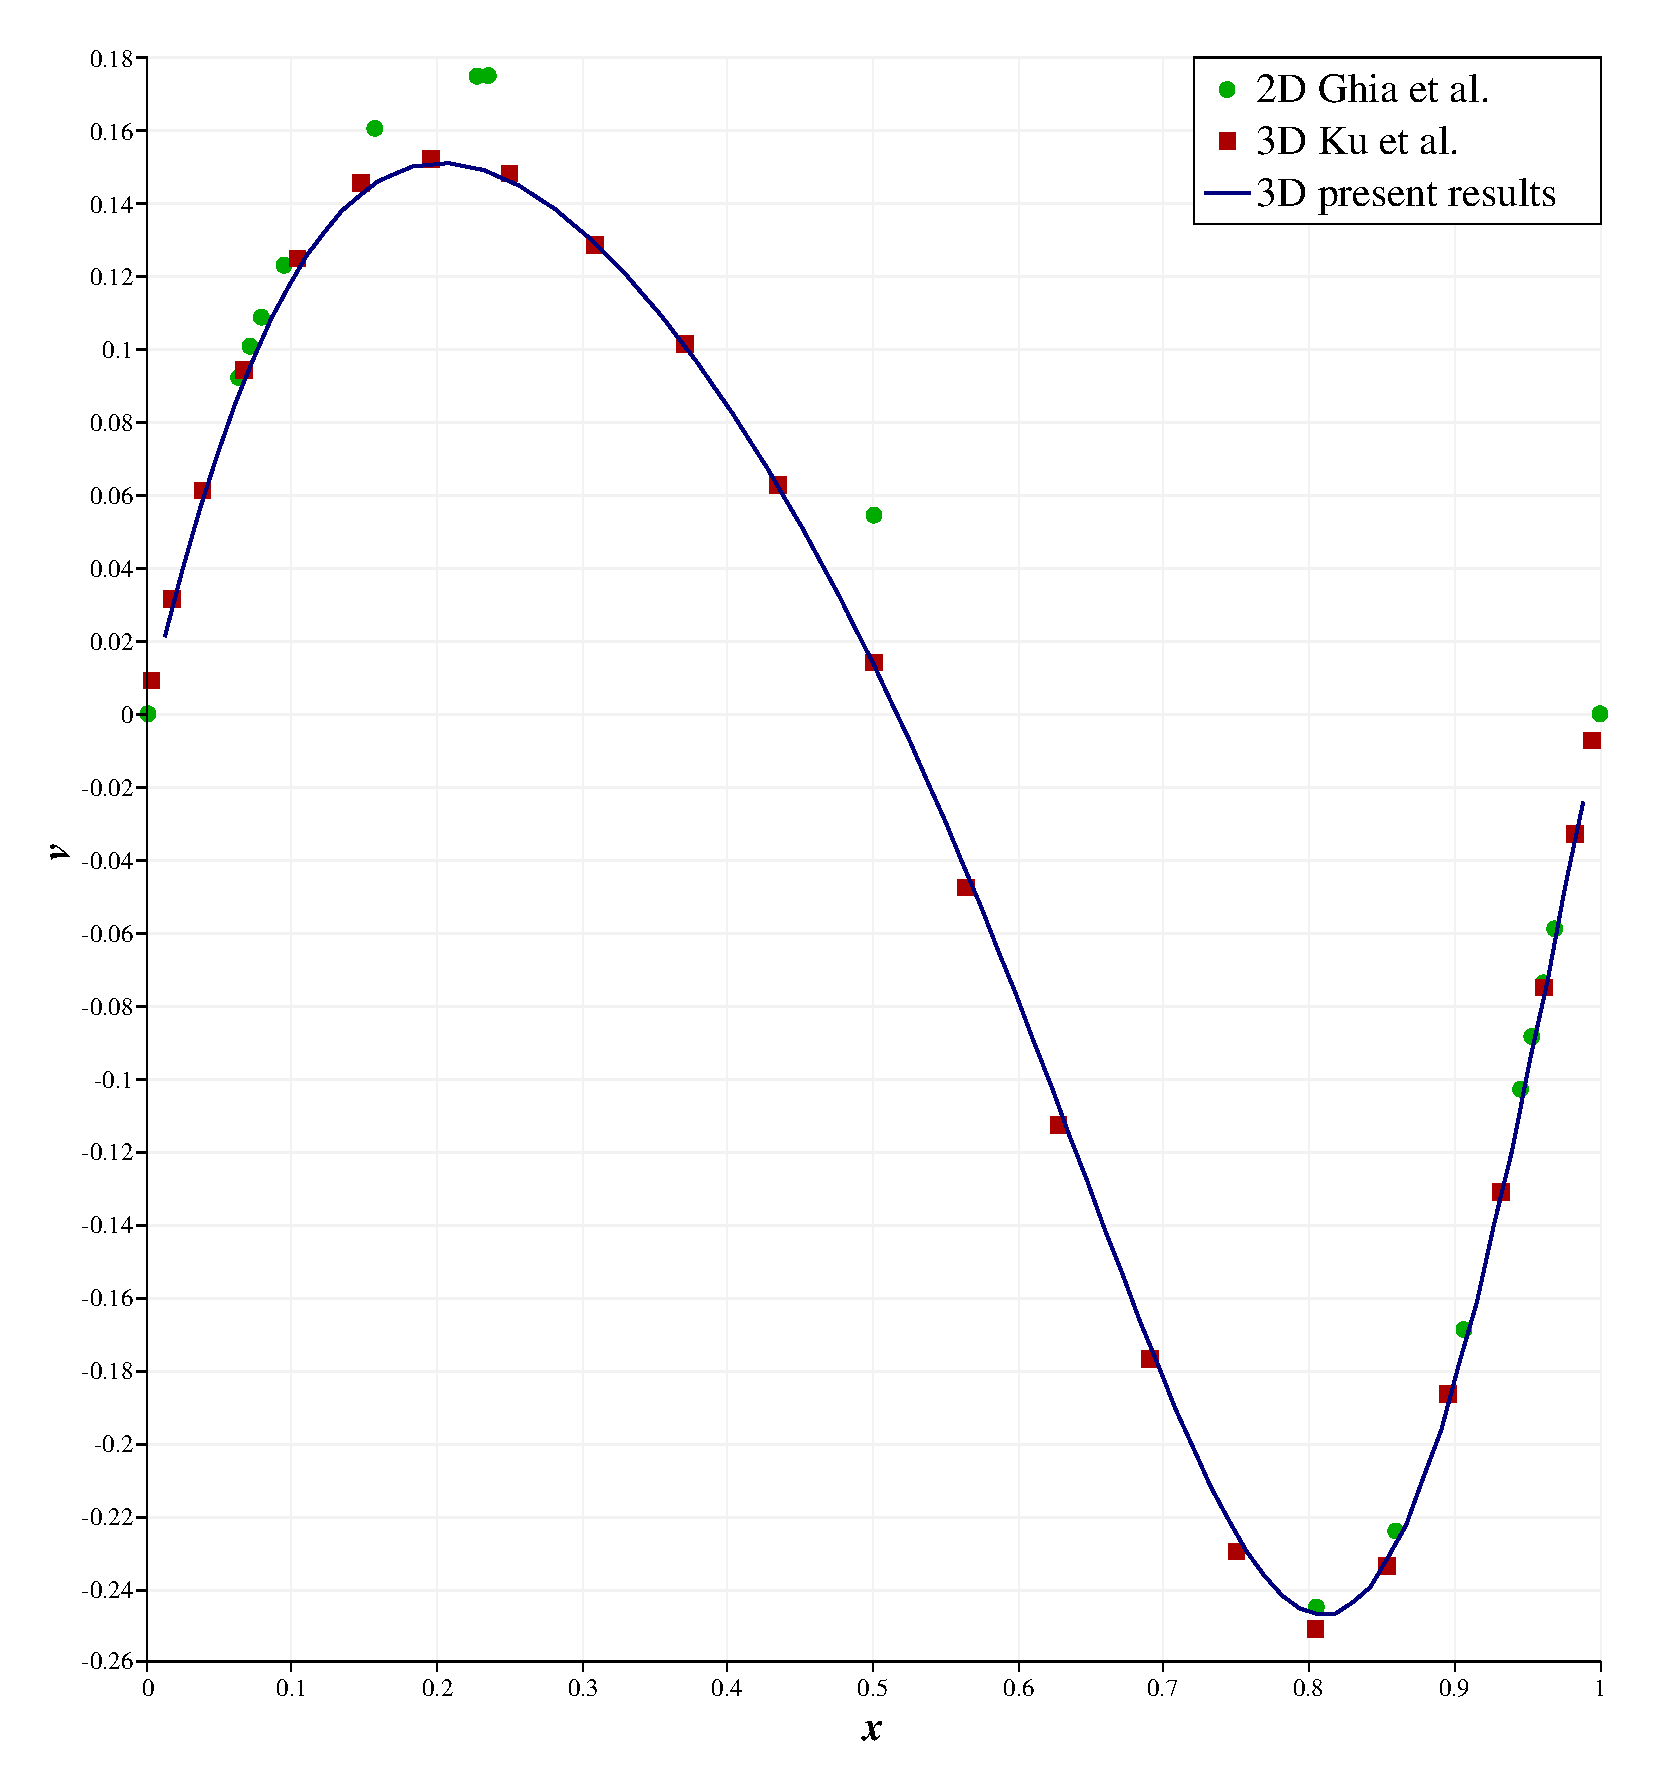
\includegraphics[width=\linewidth]{V-3D_vs_Ku-3D.eps}
    \caption{\(v\)-velocity profile on the horizontal centerline in cubic cavity (at the center of \(z\)-axis).}
\end{figure}

The results of the developed solver are in very good agreement with the three-dimensional results of Ku et al \cite{Ku:1987:PMS:33136.33145}. The differences with two-dimensional flow are apparent due to the effect of three-dimensional boundary conditions.

\newpage

\subsection{Future tasks}
\begin{enumerate}
    \item Obtain and compare results at \(\text{Re}=400\) and \(\text{Re}=1000\).
    \item Convert the 2D and 3D code for use with parallel computing using OpenMP.
\end{enumerate}

\bibliographystyle{unsrt}
\bibliography{33145.bib,0021999182900584.bib}

\end{document}
